%!TEX root=../document.tex

\section{Einleitung}
\label{sec:Einleitung}
Load Balancing ist kein neues Konzept im Server- und Netzwerkbereich. Viele Produkte, wie z.B. Router die Netzwerkverkehr über verschiedene Netzwerk Ressourcen zum gleichen Ziel verteilen, können unterschiedliche Arten des Load Balancing durchführen. Im Gegensatz zum Router wird bei Server Load Balancing der Netzwerkverkehr über verschiedene Server Ressourcen verteilt. Anfangs wurden Load Balancer als reine Lastenverteiler verwendet, doch heute sind Load Balancer schon so weit entwickelt, dass sie zusätzliche Funktionen wie Healthchecks, Optimierung von Datenflüssen, etc. zur Verfügung stellen.

Im Webhostingbereich wird Load Balancing typischerweise für die Verteilung von http-Verkehr auf mehrere Server (Nodes), bei dem der Load Balancer als Web Front-End agiert, eingesetzt. Der Load Balancer beurteilt die Antwortzeiten und Auslastung der einzelnen Server und verteilt basierend auf dieser Beurteilung die Anfragen. Durch die Verteilung des Dienstes auf mehrere Server schützt man sich zusätzlich vor Hardwareausfall, da bei Ausfall eines Server Nodes der Netzwerkverkehr einfach über andere Nodes erfolgen kann. Das primäre Ziel ist es, den Netzwerkverkehr bei hoher Nachfrage auf alle vorhandenen Nodes aufzuteilen, um die bestmögliche Performance zu gewährleisten. Der User weiß normalerweise nichts über vorhandene Backend- bzw. Backupserver, für ihn scheint es so als ob nur ein Server hinter einem Dienst steht. 
 \cite{LoadBalancing1}

\subsection{Wann und wozu verwendet man Load Balancing?}
\label{sec:Wann und wozu verwendet man Load Balancing?}

\begin{list}{•}{}
\item Failover und Redundanz

	  Ein wesentliches Einsatzgebiet des Load Balancing ist die Ausfallsicherheit und die daraus resultierenden 		  erhöhte Uptime (Betriebszeit). Durch Verwendung von mehreren identischen Nodes kann der Netzwerkverkehr im 	  Falle eines Hardware oder Softwarefehlers umverteilt werden und die Website, Dienst, etc. bleibt 			 	  verfügbar. 
\item Wachsende Nachfrage und Verfügbarkeit
	  
	  Falls die Website, Dienst, etc. so beliebt wird, dass ein einziger Server die Masse an Anfragen nicht in 			  absehbarer Zeit abarbeiten kann (was zu z.B. lange Wartezeit bei Seitenaufbau führt), sollte man ebenfalls 	  Load Balancing einsetzten. Dadurch können die Anfragen auf mehrere Server verteilt werden und so ist die 			  Verfügbarkeit wieder gegeben. \cite{LoadBalancing1}  
\end{list}

\pagebreak
\subsection{Beispiel Website}
\label{sec:Beispiel Website}
Anhand dieses kleinen Beispiels einer Website möchte ich die zwei oben genannten Haupteinsatzgründe für Load Balancing veranschaulichen. 
\begin{figure}[!ht]
	\begin{center}
		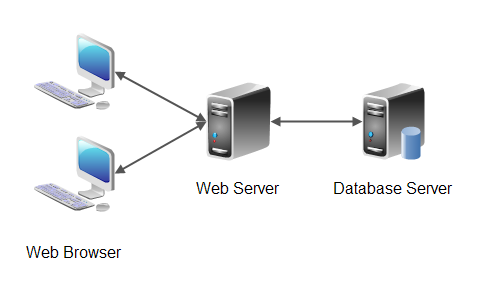
\includegraphics[width=0.4\linewidth]{images/loadbalancing12.jpg}
		\caption{Aufbau Website \cite{LoadBalancingGrafik2}}
		\label{Aufbau Website}
	\end{center}
\end{figure}

Mögliche Probleme bei einer Website: zu hohe Anzahl an Anfragen für Webserver oder Datenbank- bzw. Webserver fällt aus.

\begin{figure}[!ht]
	\begin{center}
		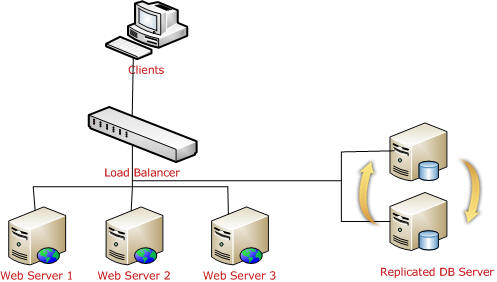
\includegraphics[width=0.4\linewidth]{images/loadbalancing1.jpg}
		\caption{Load Balancing Beispiel \cite{LoadBalancingGrafik1}}
		\label{Load_Balancing_Beispiel}
	\end{center}
\end{figure}

Lösung durch Load Balancing: Einsatz von mehreren Servern. Um für eine hohe Anzahl an Anfragen gerüstet zu sein, muss die Website über mehrere Webserver verfügbar sein. Da eine Domain nur einem physikalischen Server zugewiesen werden kann, wird der Load Balancer zwischen dem Internet und den Webservern geschaltet und bekommt die öffentliche Domain zugewiesen. Wenn mehrere User die Website abrufen, beurteilt der Load Balancer die Antwortzeiten und Auslastung der einzelnen Webserver und verteilt die Anfragen so, dass die bestmögliche Performance erreicht wird. Außerdem wird so auch die Ausfallsicherheit der Website gewährleistet, da die Website jetzt über mehrere Webserver gehostet wird. Zusätzlich wird in diesem Beispiel ein Backupserver der Datenbank erstellt. Falls der Datenbankserver ausfällt oder ausgetauscht werden muss, springt einfach der Backupserver ein.      

\pagebreak
\subsection{Notwendigkeit von Load Balancing}
\label{sec:Notwendigkeit von Load Balancing}
Das primäre Ziel von Load Balancing ist es den Netzwerkverkehr bei hoher Nachfrage auf alle vorhandenen Nodes aufzuteilen, um die bestmögliche Performance zu gewährleisten. Netzwerke und Server sind die Hauptgründe, warum Load Balancing notwendig ist. In der heutigen Zeit ist das Internet ein wichtiger Bestandteil für jedes Unternehmens (um Netzwerk zwischen Firma, Lieferanten, Kunden, etc. zu erzeugen), bei dem es auch um viel Geld geht. Firmen, vor allem im e-commerce Bereich (elektronischer Handel), können es sich nicht leisten, wenn ihr Netzwerk entweder sehr langsam ist bzw. ausfällt. 
Um z.B. eine Website für elektronischen Handel zu erstellen, muss man Faktoren wie Server, Switches, Firewalls, etc. berücksichtigen. Durch das Verwenden von mehreren Servern für so eine Website entstehen aber Herausforderungen in den Bereichen Skalierbarkeit, Verwaltbarkeit und Verfügbarkeit. Load Balancing löst zusätzlich viele dieser Probleme.
.\vspace{5mm}
\textbf{Skalierbarkeit} \\

Skalierbarkeit ist kein neues Problem. Früher ist eine Applikation auf einem Server gelaufen. Falls dieser Server für die Applikation nicht mehr ausreichend war, wurde dieser entweder verbessert oder durch einen performanteren Server ersetzt. Durch Load Balancing ist es jedoch möglich, die Applikation auf mehreren Servern zu verteilen. Durch die mehreren Server ist es möglich, sämtliche Anfragen zu verteilen um bestmögliche Performance zu gewährleisten. Load Balancer verwenden Scheduling Algorithmen um die Anfragen zu verteilen\vspace{5mm}

\textbf{Verwaltbarkeit} \\

Wenn die Serverhardware verbessert oder das Betriebssystem aktualisiertet werden muss, muss der Server abgeschaltet werden. Man kann das natürlich in der Zeit machen, in der am wenigsten Bedarf an der Website/Dienst besteht (vermutlich in der Nacht), jedoch hat man trotzdem eine Ausfallzeit (Downtime). Doch manche Firmen können sich überhaupt keine Ausfallzeit leisten oder haben konstanten Bedarf  an ihrem Service. Ein Load Balancer kann Server, die für Wartungszwecke offline gestellt werden müssen, ohne Downtime ausschalten. Das wird gewährleistet, in dem der Load Balancer keine weiteren Anfragen an diesen Server weiterleitet und wartet bis sämtliche bestehende Anfragen abgearbeitet wurden. Dann kann der Server offline gestellt werden. Sämtliche Anfragen werden auf die anderen Server weitergeleitet. Zusätzlich helfen Load Balancer beim Verwalten von Content Managementsystem, da es bei solchen Systemen ebenfalls sein kann, das ein Server nicht ausreicht.\vspace{5mm}   

\textbf{Verfügbarkeit} \\

Der Load Balancer kontrolliert kontinuierlich die Verfügbarkeit aller Server und laufenden Applikationen. Wenn der Healthcheck einer dieser Server oder Applikationen scheitert, sendet der Load Balancer keine Anfragen mehr zu diesem Server. \cite{LoadBalancing2}

\pagebreak
\subsection{Load Balancing Applikationen}
\label{sec:Load Balancing Applikationen}
\textit{"With the advent of the Internet, the network now occupies center stage. As the Internet connects the world and the intranet becomes the operational backbone for businesses, the IT infrastructure can be thought of as two types of equipment: computers that function as a client and/or a server, and switches/routers that connect the The Network Environment computers. Conceptually, load balancers are the bridge between the servers and the network, as shown in the graphic below. On one hand, load balancers understand many higher layer protocols, so they can communicate with servers intelligently. On the other, load balancers understand networking protocols, so they can integrate with networks effectively"}  \cite{LoadBalancing2}

\begin{figure}[!ht]
	\begin{center}
		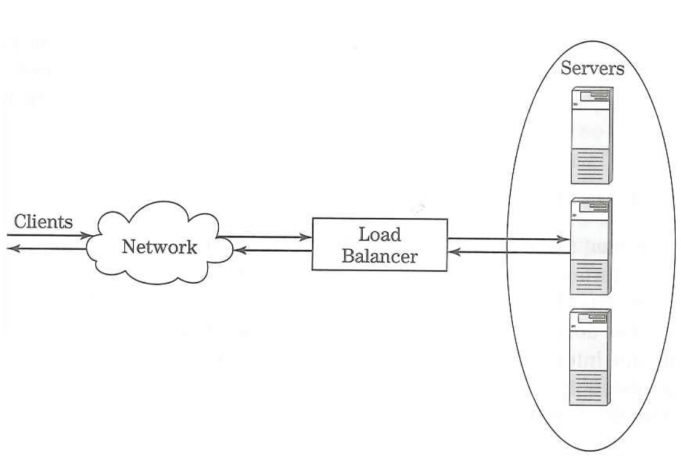
\includegraphics[width=0.6\linewidth]{images/loadbalancing2.jpg}
		\caption{Load Balancing einer Serverfarm \cite{LoadBalancing2}}
		\label{Load Balancing einer Serverfarm}
	\end{center}
\end{figure}

Load Balancer haben zumindest vier Applikationen:
\begin{list}{•}{}
\item Server Load Balancing
\item Global Server Load Balancing
\item Firewall Load Balancing
\item Transparent Cache Switching
\end{list}

Server Load Balancing: Verteilung der Anfragen auf mehrere Server um die Auslastung gleichmäßig zu verteilen und um sich vor Serverausfall zu schützen

Global Server Load Balancing: Verteilung der User zu verschiedenen Data Center, die aus Serverfarmen bestehen für schnelleren Rückmeldung und als Schutz vor Data Center Ausfällen.

Firewall Load Balancing: Verteilung des Netzwerkverkehrs auf mehrere Firewalls um vor Firewallausfall geschützt zu sein.

Transparent Cache Switching: lenkt den Netzwerkverkehr zu Caches um den Antwortzeit zu verringern. 

\textbf{Load Balancing Produkte} \\

Load Balancing Produkte können in 3 Kategorien unterteilt werden: Softwareprodukte,  Switches und  Geräte

Software Load Balancing Produkte laufen direkt auf den Load-Balancer Servern. Die Software führen die Algorithmen aus, welche für die Lastverteilung zuständig sind. Beispiele für Software Load Balancing Produkte sind z.B. Incapsula, NGINIX und BalanceNG 

Switches haben ihre normalen Funktionalitäten auf OSI Layer 2/3, doch können zusätzlich Load Balancen auf Layer 4-7. Das wird durch zusätzliche Hardware oder Software erreicht.  

Geräte sind Blackbox Produkte, welche die notwendige Hardware und Software für Web Switching besitzen. Das könnte z.B. ein einfacher Computer oder Server mit speziellem Betriebssystem und spezieller Software sein. \cite{LoadBalancing2}

\subsection{Konfiguration eines Load Balancers}
\label{sec:Konfiguration eines Load Balancers}

\begin{figure}[!ht]
	\begin{center}
		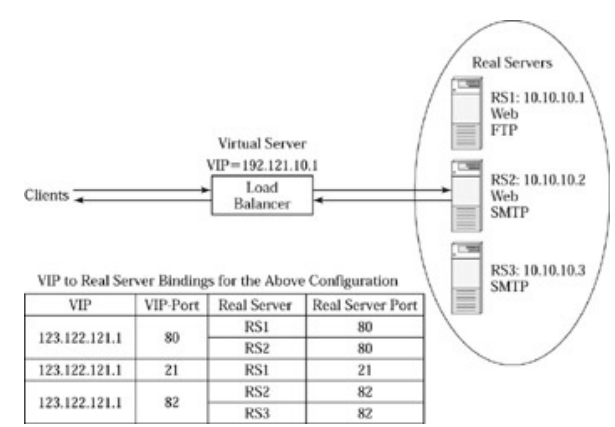
\includegraphics[width=0.6\linewidth]{images/loadbalancing8.jpg}
		\caption{Load Balancing Konfiguration \cite{LoadBalancing2}}
		\label{Load Balancing Konfiguration}
	\end{center}
\end{figure}
\begin{enumerate}
\item virtuelle IP (VIP) des Load Balancers definieren: VIP = 123.122.121.1
\item Applikationen definieren, die Load Balancing benötigen: Web, FTP und SMTP
\item Bei jeder Applikation muss die virtuelle IP mit jedem realen Server verbunden werden, auf dem diese Applikation läuft
\item Arten der Healthchecks am Load Balancer konfigurieren, nach denen der Zustand der Server bestimmt werden soll
\item Sheduling Algorithmus konfigurieren, nach dem die Last verteilt wird \cite{LoadBalancing2}
\end{enumerate}

\section{Algorithmen zur Lastenverteilung}
\label{sec:Algorithmen zur Lastenverteilung}
Load Balancer können verschiedene Algorithmen verwenden, um Lasten jedem Server in einer Serverfarm zuzuweisen. Die folgenden Algorithmen können hierzu verwendet werden.

\subsection{Round-Robin}
\label{sec:Round-Robin}
Round-Robin ist das einfachste Verfahren zur Lastenverteilung.
Ein Load Balancer weist jedem Server der Reihe nach eine Verbindung zu.
Dieses Verfahren kann eine gleichmäßige Verteilung der Last nicht sicherstellen, da jede Verbindung über unterschiedliche lange Zeiträume bestehen kann. Infolgedessen können manche Server mehr gleichzeitig aktive Verbindungen haben, als andere. \cite{LoadBalancing2}
Da bei diesem Algorithmus dieser Aspekt nicht bedacht wird, kann eine schlechte Lastverteilung auftreten. Hardwaretechnisch schwächer ausgestattete Server könnten so mit Anfragen überladen werden.

Da Round-Robin eine sehr einfache Methode zur Lastverteilung ist, werden sehr wenige Ressourcen seitens des Load Balancers benötigt. Infolgedessen ist der Algorithmus nur dann sehr effektiv, wenn der Lastverteilungsalgorithmus viel Rechenzeit benötigt.
Soll beispielsweise aus 1000 Servern der nächstbeste Server ausgewählt werden, so würde dies bei anderen Algorithmen einen erhöhten Rechenaufwand seitens der Load Balancers bedeuten. Dieser Algorithmus würde sich besonders in Situation anbieten, in denen die Art, und daraus resultierende Last am Server, und Dauer der Anfrage in etwa gleich bleiben, da so eine gleichmäßige Verteilung gewährleistet werden kann. \cite{LoadBalancing2}

\subsection{Least Connections}
\label{sec:Least Connections}
Jede neue Anfrage wird dem Server mit den geringsten gleichzeitig aktiv vorhandenen Verbindungen zugesandt. Der Load Balancer muss hierbei die Anzahl dieser Verbindungen jedes Servers jederzeit festhalten. Diese Methode ist eine der effektivsten und beliebtesten in verschiedenen Anwendungsbereichen, wie beispielsweise DNS oder dem Web. Der Hauptgrund hierfür sind das einfache Verstehen und Anwenden der Methode. \cite{LoadBalancing2}

Least Connections kann dann von Nutzen sein, wenn zwei oder mehr Server mit gleicher Ausstattung unterschiedlich stark belastet werden. Dies ließe sich beispielsweise auf eine unterschiedliche Dauer von Sessions der Benutzer zurückzuführen.
\cite{WeightedLoadBalancingGrafik}

\subsection{Weighted Distribution}
\label{sec:Weighted Distribution}
Da verschiedene Server hardwaretechnisch verschieden ausgestattet sein können, kann mithilfe dieser Methode eine Angabe der Leistung der einzelnen Server in Relation zueinander erfolgen, indem jedem Server eine gewisse Gewichtung zugewiesen wird. Der Load Balancer kann so beispielsweise bei einer durch einen Serveradministratoren festgelegten Gewichtung von 5-1 dem 1. Server 5 mal so viele Anfragen zukommen lassen, wie dem 2. Die Verteilung ist der Abbildung 4 zu entnehmen.

\begin{figure}[!ht]
	\begin{center}
		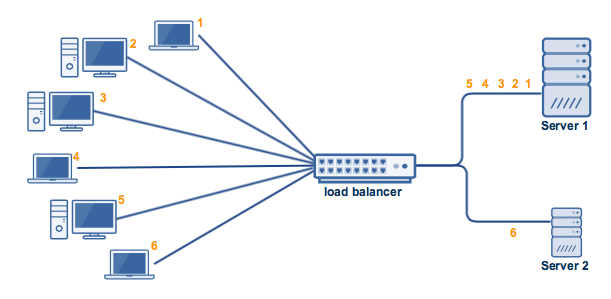
\includegraphics[width=0.8\linewidth]{images/weighted_round_robin.png}
		\caption{Weighted Distribution anhand von Weighted Round-Robin \cite{WeightedLoadBalancingGrafik}}
		\label{Weighted Round-Robin}
	\end{center}
\end{figure}

In der Praxis wird diese Methode in Kombination mit anderen Methoden, wie Least Connections oder Round-Robin angewandt.
Sollen nun weitere Server hinzugefügt werden im Fall von Weighted Round-Robin die Anfragen wie gewohnt der Reihe nach gewichtet verteilt. Im Fall von Weighted Least Connections ist lediglich auf die Anzahl der aktuell verbundenen Clients und die Gewichtung zu achten. Um eine gerechte Verteilung der Last zu gewährleisten, wird die Anzahl der aktiven Verbindungen durch die Gewichtung dividiert.

Diese Methode ist besonders dann geeignet, wenn bereits bestehende, womöglich leistungsschwächere Hardware mit leistungsstärkerer kombiniert werden soll.
\cite{LoadBalancing2}

\subsection{Response Time}
\label{sec:Response Time}
In der Annahme, dass eine schnelle Reaktion eines Servers eine gute Performance zur Folge hat, wird die Reaktionszeit eines Servers vom Load Balancer gemessen und anhand dieser ein Server ausgewählt. Hierzu werden entweder HTTP GET oder TCP SYN (Synchronize) Anfragen versandt und die Zeit gemessen, die vergeht, bis eine HTTP GET Antwort oder TCP SYN ACK (Synchronize Acknowledge) von diesem Server zurückgekommen ist. \cite{LoadBalancing2}

\begin{figure}[!ht]
	\begin{center}
		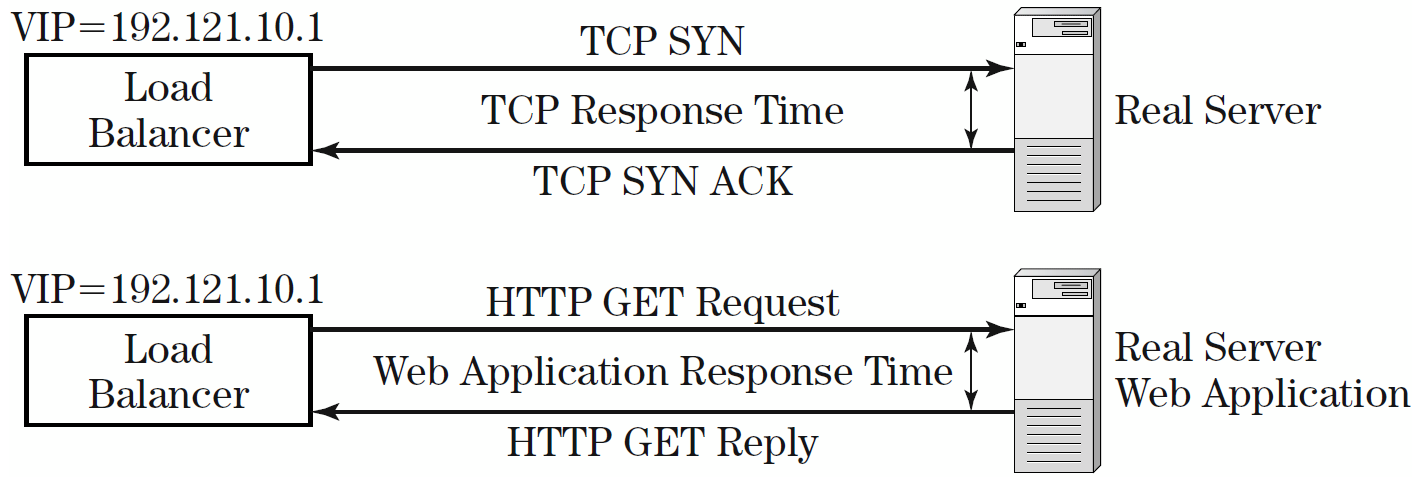
\includegraphics[width=0.8\linewidth]{images/LoadBalancing_Response_Time.png}
		\caption{Messen der Zeit, die der Server für eine Antwort benötigt \cite{LoadBalancing2}}
		\label{ResponseTime}
	\end{center}
\end{figure}

Für eine effiziente Lastenverteilung muss diese Antwortzeit über einen längeren Zeitraum gemessen werden, da die aktuellen Zeiten nicht mehr den Zeiten von vor beispielsweise einer Stunde entsprechen müssen. Der Load Balancer kann, basierend auf vergangenen, aber auch aktuellen Messungen, berechnen, welcher Server als Nächstes am Schnellsten antworten könnte.

Aufgrund der Komplexität dieser Methode, könnte diese Methode alleine nicht die beste Möglichkeit zur Lastenverteilung bieten. Der Algorithmus kann hingegen in Kombination mit anderen Load Balancing Methoden funktionieren. \cite{LoadBalancing2}

\subsection{Server-Probe}
\label{sec:Server-Probe}
Auf jedem Server rennt im Hintergrund ein Programm, welches die aktuelle Auslastung des Servers an den Load Balancer in regelmäßigen Zeitabständen weiterleitet. Auf diese Weise hat der Load Balancer stets Zugriff auf Daten, wie die aktuelle Auslastung der CPU, aber auch den verfügbaren Arbeits- und Festplattenspeicher.
Ein wesentlicher Nachteil dieser Methode ist die Entwicklung und Installation von zusätzlicher Software, die mit der auf dem Server laufenden Applikation lauffähig sein muss, ohne die Anwendung selber zu beeinflussen. Es ist auch ungewiss, ob solche Messungen die genaue Serverauslastung dokumentieren, da es einen leistungstechnischen Flaschenhals auch an anderer Stelle geben kann, wie beispielsweise die Zugriffsgeschwindigkeit der Festplatte des Servers auf die Daten oder den Datendurchsatz der Netzwerkkarte. \cite{LoadBalancing2}

\subsection{Kombiniert}
\label{sec:Kombiniert}
Die Kombination von zwei oder mehreren Methoden kann eine besseres Erfassen der Serverlast ermöglichen. Hierzu können beispielsweise die Methoden Response Time und Least Connections zusammen verwendet werden. Die Verfahren können vom Load Balancer wieder mit entsprechender Gewichtung verwendet werden. \cite{LoadBalancing2}

\subsection{Server Load Thresholds}
\label{sec:Server Load Thresholds}
Server haben die Tendenz dazu bis zu einem gewissen Punkt bzw. Schwellenwert leistungstechnisch gut zu funktionieren. Sollte dieser Schwellenwert überschritten werden, so wird dieser Server seine Daten aus dem Arbeitsspeicher auf der Festplatte auslagern oder der Prozessor überlastet sein, was einen signifikanten Einbruch in der Leistung des Servers zur Folge hat.

\begin{figure}[!ht]
	\begin{center}
		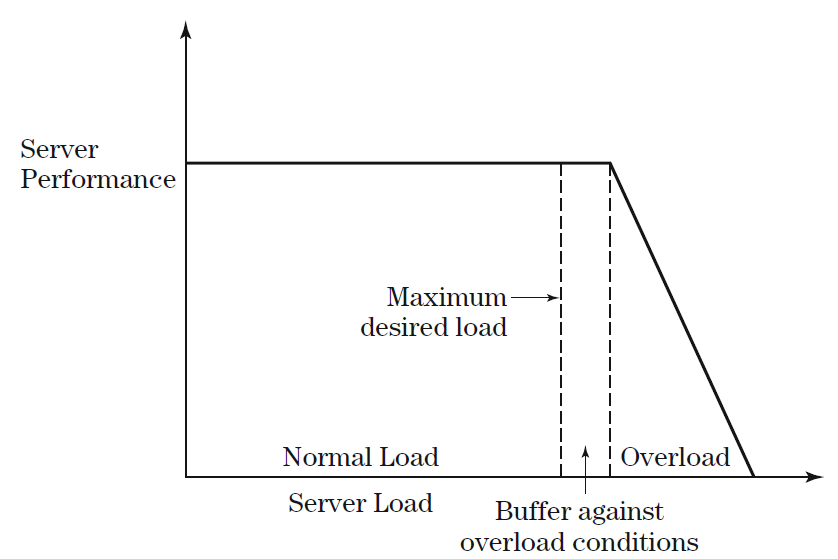
\includegraphics[width=0.5\linewidth]{images/LoadBalancing_LoadThreshold.png}
		\caption{Optimieren der Serverleistung \cite{LoadBalancing2}}
		\label{ServerTheshold}
	\end{center}
\end{figure}

Um den Server vor weiteren neuen Zugriffen zu schützen (und ihn nicht noch weiter zu belasten) wird ein Schwellenwert seitens des Load Balancers festgelegt, der knapp unter dem Grenzwert liegt, der den Server leistungstechnisch an seine Grenzen bringen würde. \cite{LoadBalancing2}

\subsection{Zufällig}
\label{sec:Zufällig}
Der zu verwendende Server wird von einem Zufallszahlengenerator am Load-Balancer festgelegt. Sollten nun innerhalb eines kurzen Zeitraumes viele Anfragen zustande kommen, so werden diese zufällig verteilt, was in etwa eine gleichmäßige Verteilung der Anfragen gewährleistet.
Diese Methode kann besonders dann verwendet werden, wenn die Server eine gleiche oder sehr ähnliche Hardwarekonfiguration haben. \cite{WeightedLoadBalancingGrafik}

\subsection{Gegenüberstellung}
\label{sec:Gegenüberstellung}
Da bei der Lastenverteilung auf einige Aspekte, wie die Auslastung der Serverhardware und Netzwerkkomponenten, die Sitzungsdauer und Inhalte dieser und inwiefern welche Komponenten wie stark ausgelastet werden, die Antwortgeschwindigkeit, ... geachtet werden muss, gibt es keinen optimalen Algorithmus zur Lastenverteilung. \cite{LoadBalancing2}

Round-Robin lässt sich vielseitig einsetzen und bietet sich besonders in Situationen an, in denen die durch die Anfrage bedingte Serverlast möglichst gleich ausfällt.
 
Least Connections wäre von Vorteil, wenn sich die Art der Anfrage stark ändern kann, wo Round-Robin im Laufe der Zeit Anfragen ungleich verteilen würde.

Eine gewichtete Verteilung kann die Anfragen auf leistungsschwächere Server in einem Cluster fair aufteilen. Die Methode bietet sich dann an, wenn bereits bestehende, in die Jahre gekommene Hardware weiterverwendet werden soll.

Response Time würde sich in Situationen anbieten, in denen zeitkritische Anwendungen ausgeführt werden müssen. Gegen die Methode spricht der erhöhte Rechenaufwand, der für die aufwändige Serverfindung benötigt wird.

Server-Probe ist dann zu verwenden, wenn eine genaue Erfassung der Serverlasten vom Load Balancer gewünscht ist, zwecks präziserer Lastenverteilung. Der entscheidende Nachteil ist, dass hierfür im Normalfall zusätzliche Software zur Erfassung der gewünschten Daten benötigt wird und durch die andauernde Kommunikation der Server mit dem Load Balancer zusätzlicher Verkehr im Netzwerk entsteht.

Server Load Thresholds können Schutz vor Serverüberlastungen bieten, die bei einem plötzlich auftretenden Ansturm auf den Server auftreten können.

In der Praxis kommt es ganz auf die Hardwareausstattung der verwendeten Server und die darauf ausgeführten Applikationen an.


\section{Caches}
\label{sec:Caches}

\subsection{Grundlagen}
\label{sec:Grundlagen}
Ein Cache ist ein schneller Zwischenspeicher, in dem häufig aus dem Internet abgerufene Dateien gespeichert werden. Es soll durch ein Zwischenspeichern von Daten die Reaktionszeit auf eine Anfrage reduziert werden. Hierbei kann auch Bandbreite gespart werden, da die Ressource, sofern sie erneut benötigt wird, nicht vom ursprünglichen Quellserver angefragt werden muss, sondern aus dem Cache geladen werden kann.
Anhand der folgenden Grafik soll die Funktionsweise eines Caches erklärt werden:

\begin{figure}[!ht]
	\begin{center}
		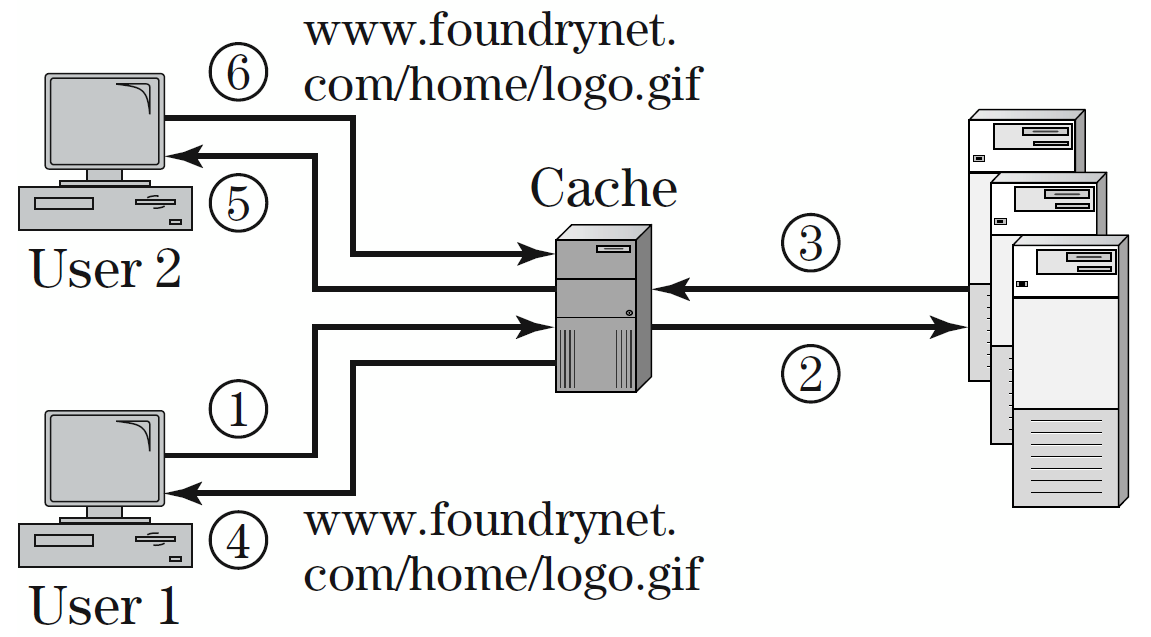
\includegraphics[width=0.5\linewidth]{images/Cache_Funktionsweise.png}
		\caption{Funktionsweise eines Caches, Zwischenspeichern einer Grafik \cite{LoadBalancing2}}
		\label{Cache_Funktionsweise}
	\end{center}
\end{figure}

Client 1 möchte die Webseite \textit{foundrynet.com} aufrufen und muss dazu, unter anderem, deren Logo herunterladen.
Es wird eine HTTP Anfrage an den Cache gesendet.
Da der Cache zum ersten Mal eine Anfrage für diese Webseite bekommt und den Content nicht zwischengespeichert hat, sendet er eine Anfrage an den Server, auf dem die Webseite gespeichert ist und sichert den durch Client 1 angefragten Content lokal im Arbeitsspeicher oder auf einer Festplatte.
Der Cache übermittelt abschließend dem Client die Webseite.
Möchte nun Client 2 ebenfalls \textit{foundrynet.com} aufrufen, so muss nur eine Anfrage an den Cache geschickt werden, der die Webseite nun lokal vorliegen hat und kann dem Client diese Version schicken, ohne den Server erneut kontaktieren zu müssen.
In Folge dessen hat Benutzer 2 den Content schneller vorliegen und es wird Bandbreite gespart. \cite{LoadBalancing2}

Da Anfragen vom Cache im Namen des Clients getätigt werden, werden solche Caches auch \textit{Proxy Cache} oder \textit{Proxy Server} genannt.
Befindet sich eine angeforderte Ressource im lokalen Speicher des Caches, so wird dies ein \textit{cache hit} genannt. Sollte dies nicht der Fall sein, so wird dies ein \textit{cache miss} genannt.
Die Effizienz eines Caches kann anhand der \textit{Cache-hit Rate} gemessen werden. Sie gibt an, wie viel Content (in Prozent) der Cache selber zur Verfügung stellt. Je höher dieser Prozentsatz ist, umso besser wirkt sich das auf die Antwortzeit aus.
\cite{LoadBalancing2}

\subsection{Cachetypen}
\label{sec:Cachetypen}
Caches können zur Beschleunigung der Antwortzeit seitens des Benutzers, aber auch zur Verbesserung der Leistung von Webservern verwendet werden. Infolgedessen kann hier zwischen zwei Typen unterschieden werden: \textit{Client-} und \textit{Serverseitige Beschleunigung}.

Auf Clientseite sollen eine raschere Antwortzeit und eine Bandbreitenersparnis ermöglicht werden. Auf Serverseite sollen eine schnellere Bereitstellung von Inhalten und eine Ersparnis an Webservern ermöglicht werden. Die Idee dahinter ist es den Cache primär zur Bereitstellung von statischem Content zu verwenden, da Caches speziell für diese Aufgabe geeignet sind. Webserver können so entlastet und nur zur Generierung von Bereitstellung von dynamischen Inhalten verwendet werden. \cite{LoadBalancing2}

\subsubsection{Client: Forward Proxy}
\label{sec:Client: Forward Proxy}
Hierbei wird explizit ein Cache-Server als Proxy einer Gruppe von Clients zugewiesen. Jeder Client muss in seinem Browser eine entsprechende Konfiguration vornehmen, um den Proxy Server verwenden zu können. Da der Proxy Anfragen im Namen des Clients stellt, können Netzwerkadministratoren nur den Proxy-Servern einen Zugriff ins Internet erlauben, was eine erhöhte Netzwerksicherheit zur Folge hat, besonders, da der Server, von dem der Content geladen wird, nur die IP-Adresse vom Cache-Server sieht.

\begin{figure}[!ht]
	\begin{center}
		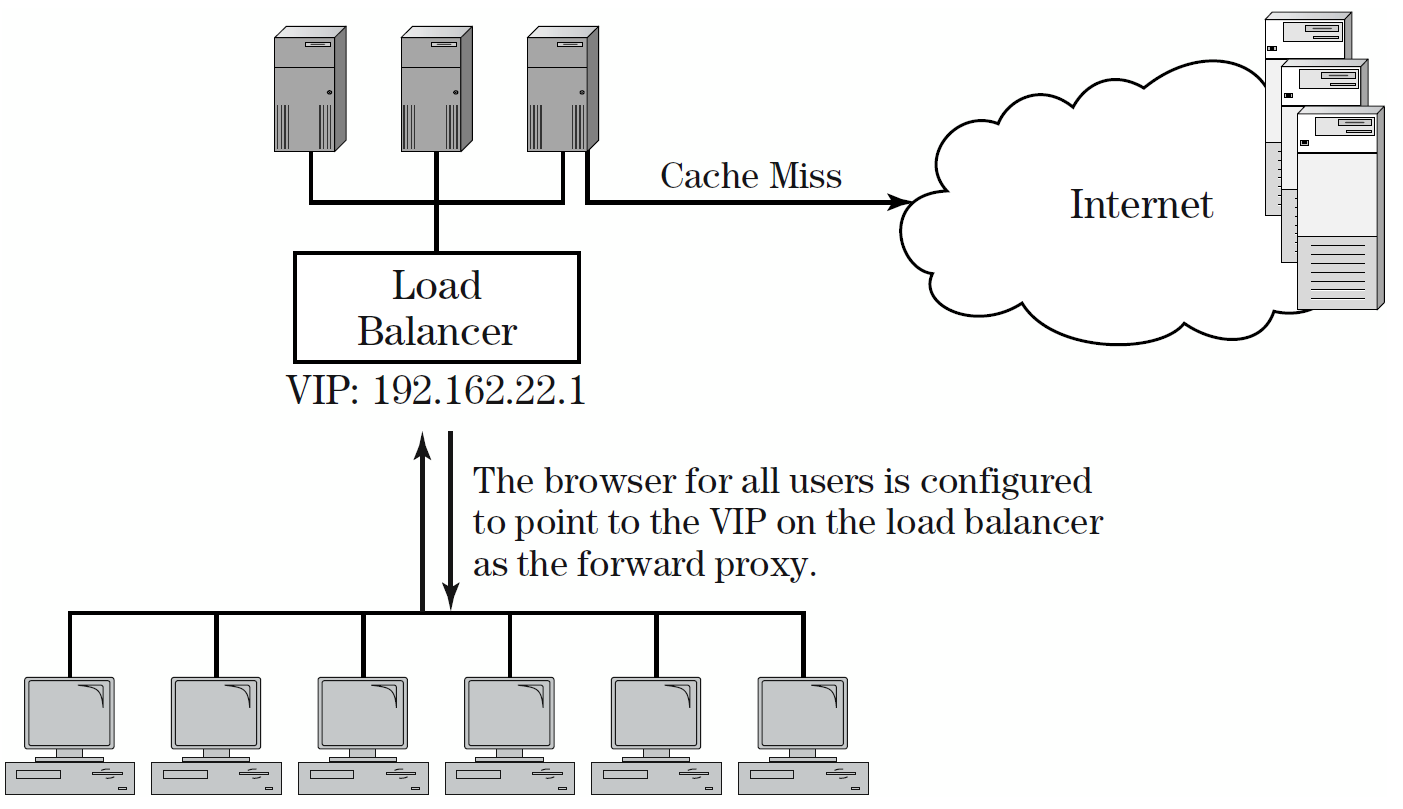
\includegraphics[width=0.5\linewidth]{images/Forward_Proxy.png}
		\caption{Funktionsweise von Forward Proxy Load Balancing \cite{LoadBalancing2}}
		\label{Forward_Proxy_Load_Balancing}
	\end{center}
\end{figure}

Um das Problem der Skalierbarkeit und Verfügbarkeit zu lösen, wird noch ein Load-Balancer zwischen die Clients und Cache-Server geschaltet und der Load-Balancer statt den Cache-Servern direkt angesprochen.
\cite{LoadBalancing2}

\subsubsection{Server: Reverse Proxy}
\label{sec:Server: Reverse Proxy}
Hierbei wird ein Cache-Server vor die Webserver geschaltet, der bei einem cache-miss direkt vor Ort die benötigten Inhalte der Webseite anfordern kann. Wichtig dabei ist, dass die Domain der Webseite nicht mehr auf die IP des Webservers, sondern des Cache-Servers zeigt.

\begin{figure}[!ht]
	\begin{center}
		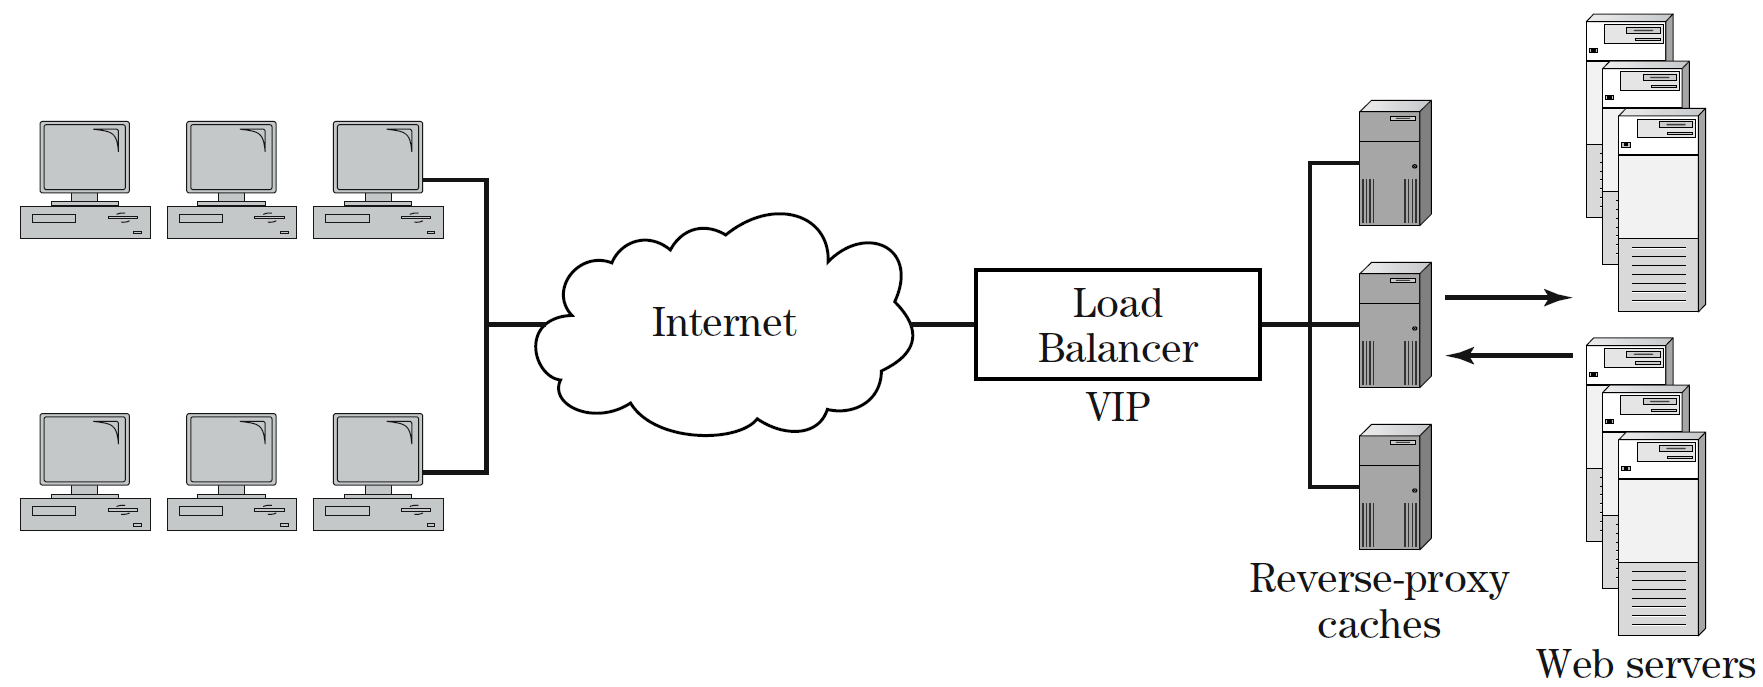
\includegraphics[width=0.5\linewidth]{images/Reverse_Proxy.png}
		\caption{Funktionsweise von Reverse Proxy Load Balancing \cite{LoadBalancing2}}
		\label{Reverse_Proxy_Load_Balancing}
	\end{center}
\end{figure}

Um das Problem der Skalierbarkeit und Verfügbarkeit zu lösen, kann auch hier noch ein Load-Balancer vor die Cache-Server geschaltet werden. Die Domain muss dann auf die externe IP des Load-Balancers gemappt werden.
\cite{LoadBalancing2}

\section{Queues}
\label{sec:Queues}
Queues (Warteschlangen) sind ein Möglichkeit, um Schreibvorgänge effizient zu verwalten. Einfache Systeme, wo der Rechenaufwand bei Anfragen und die Datenbank klein sind, sollten Schreibvorgänge schnell abgearbeitet sein. Sobald ein System aber umfangreicher, komplexer wird, können solche Vorgänge einen längeren Zeitraum in Anspruch nehmen. Die Daten könnten auch an mehreren Stellen geschrieben werden, während die Serverlast hoch ist, was eine schlechte Performance zur Folge hat.
\cite{Queues}

Die folgende Grafik visualisiert ein System ohne Queues:
\begin{figure}[!ht]
	\begin{center}
		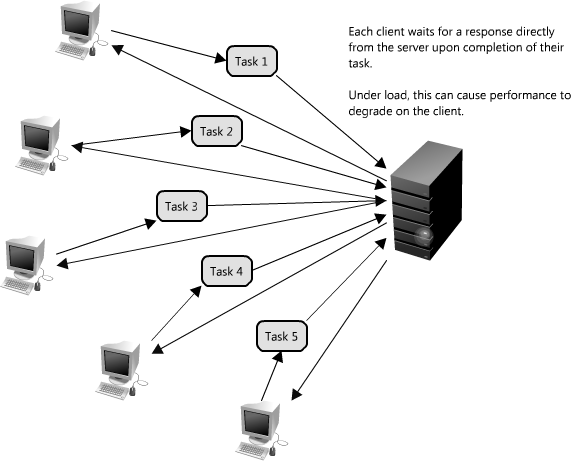
\includegraphics[width=0.5\linewidth]{images/synchronousRequest.png}
		\caption{System ohne Queues \cite{Queues}}
		\label{System_ohne_Queues}
	\end{center}
\end{figure}

Die Clients müssen auf eine Antwort des Servers warten, bevor sie mit ihrer Tätigkeit fortfahren können. Dieses synchrone Verhalten vermindert die Leistung des Clients sehr. Die Lösung für dieses Problem sind Queues. Sie trennen die Anfragen des Clients von der eigentlichen Tätigkeit, die vom Server verrichtet werden soll.

\begin{figure}[!ht]
	\begin{center}
		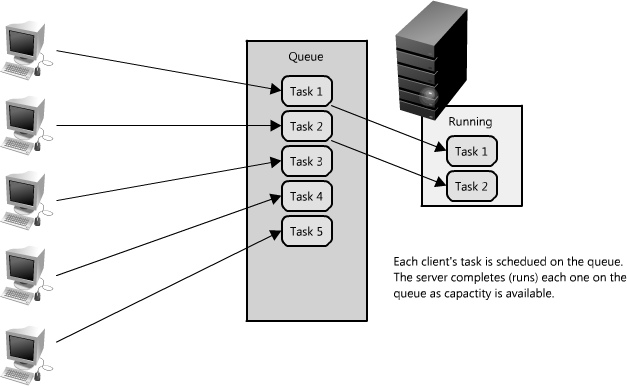
\includegraphics[width=0.5\linewidth]{images/queues.png}
		\caption{System ohne Queues \cite{Queues}}
		\label{System_mit_Queues}
	\end{center}
\end{figure}

Wie auf der Abbildung zu erkennen ist, werden Anfragen einfach der Reihe nach eingeordnet und vom Server abgearbeitet. Queues ermöglichen es dem Client eine asynchrone Weise zu arbeiten, da sie nicht auf eine Antwort vom Server warten müssen.
Der Client bekommt eine Bestätigung, dass der Task erhalten wurde und er kann in regelmäßigen Abständen überprüfen, ob der Task bereits abgearbeitet wurde.
\cite{Queues}

\section{Probleme}
\label{sec:Probleme}

\subsection{Mega Proxy Session}
\label{sec:Mega Proxy Session}
Die Mega Proxy Session, auch bekannt als Mega Proxy Problem tritt auf, wenn die korrekte IP-Adresse eines Clients nicht ermittelbar ist. Dieses Problem kann auftreten, wenn sich der Client hinter einem Proxy-Server befindet und dieser die IP-Adresse des Clients auf seine eigene ändert und der Zielserver nur mehr diese sehen kann. Die meisten ISP und Firmen haben einen oder mehrere Proxy-Server in ihrem Netzwerk, um die Identität des Clients zu verschleiern. Dabei kann es zu einem Problem mit der Sitzungspersistenz und in Folge dessen auch zu einem Load-Balancing Problem beim Load-Balancer kommen. Um dieses Problem vermeiden zu können, kann der Load-Balancer die Clients nicht mehr nur auf IP-Basis identifizieren. Das Load-Balancing Konzept muss verändert werden.

\begin{figure}[!ht]
	\begin{center}
		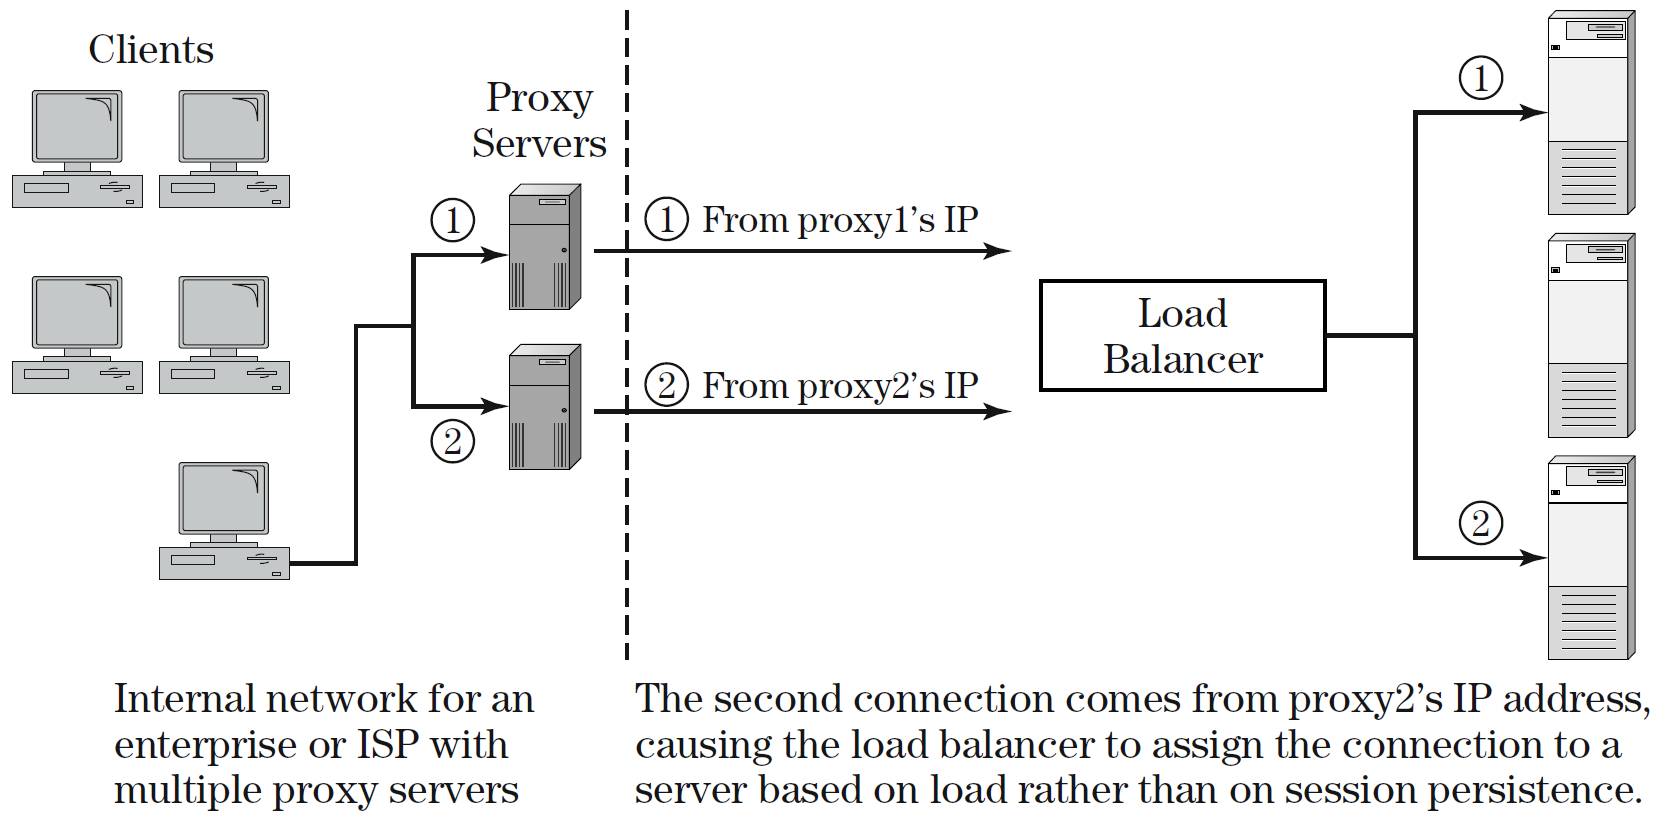
\includegraphics[width=0.5\linewidth]{images/MegaProxy1.png}
		\caption{Sitzungspersistenzproblem bei Megaproxy \cite{LoadBalancing2}}
		\label{Sitzungspersistenzproblem_bei_Megaproxy}
	\end{center}
\end{figure}

Die virtuelle Quell-IP-Adressen könnten gruppiert und als ein Server behandelt werden. Auf diese Weise ist der Load-Balancer immer noch in der Lage die Sitzungspersistenz aufrechterhalten zu können, indem alle Anfragen zu einem Server geleitet werden.
Einerseits wird das Problem bezüglich der Sitzungspersistenz gelöst, andererseits kann das Lastverteilungskonzept fehlschlagen, da alle Anfragen des Proxy-Netzwerkes an den gleichen Server weitergeleitet werden.
\cite{LoadBalancing2}

\begin{figure}[!ht]
	\begin{center}
		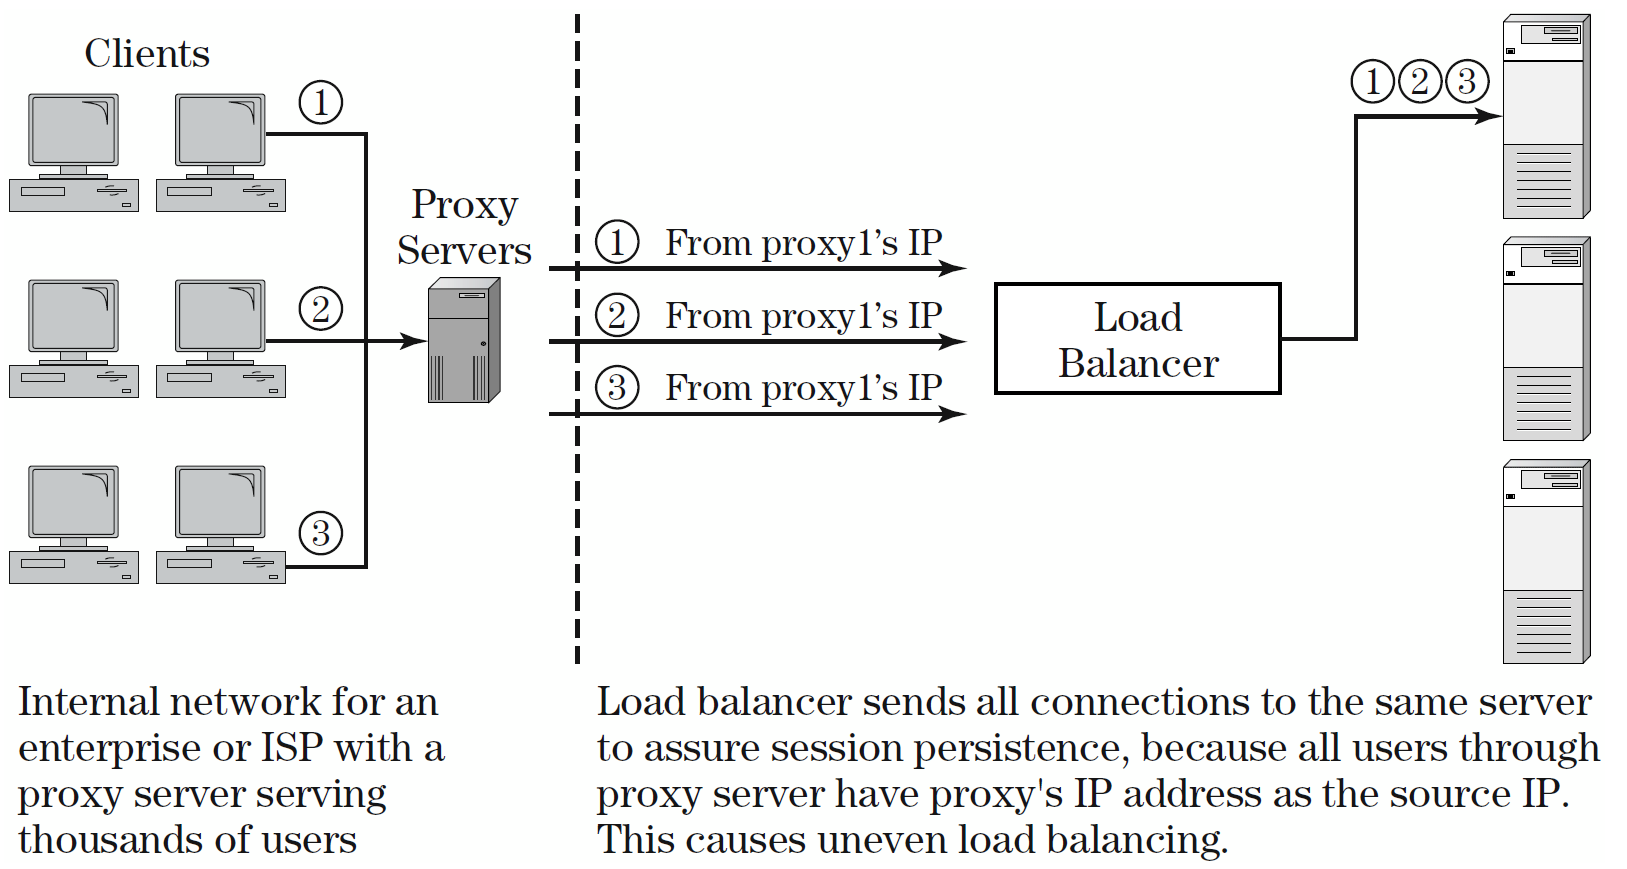
\includegraphics[width=0.5\linewidth]{images/MegaProxy2.png}
		\caption{Load-Balancing Problem bei Megaproxy \cite{LoadBalancing2}}
		\label{Load-Balancing_Problem_bei_Megaproxy}
	\end{center}
\end{figure}

\section{Apache Hadoop}
\label{sec:Apache Hadoop}
Apache Hadoop ist ein Framework, welches das verteilte Verarbeiten von großen Datenmengen, die auf vielen Clustern verstreut sein können. Das Design erlaubt es, dass sowohl ein paar wenige, aber auch mehrere 1000 Server mühelos verwendet werden können. Das Framework selbst wurde so entworfen, dass Fehler auf Applikationsebene entdeckt und beseitigt werden können, was wiederum eine hohe Verfügbarkeit des Services auf dem Cluster sicherstellt. \cite{Hadoop1}

\subsection{Module}
\label{sec:Module}
\textbf{Hadoop Common:} Werkzeuge, um die andere Hadoop Module unterstützen zu können.

\textbf{Hadoop Distributed File System (HDFS™):} Ein verteiltes Dateisystem mit einer hohen Datendurchsatzrate

\textbf{Hadoop YARN:} Ein Framework zur Aufgabenverwaltung und Verwaltung von Clusterressourcen

\textbf{Hadoop MapReduce: } Ein System, welches auf YARN basiert und zur paralellen Verarbeitung von großen Datenmengen dient

\cite{Hadoop1}

\subsection{Einsatzgebiete}
\label{sec:Einsatzgebiete}
Hadoop wird unter anderem von, Adobe, AOL, EBay, Facebook, Google, Hulu, IBM und vielen anderen Firmen verwendet.
\cite{Hadoop2}

\section{Networking Grundlagen}
\label{sec:Networking Grundlagen}

\subsection{OSI Schichtenmodell}
\label{sec:OSI Schichtenmodell}
Das OSI Schichtenmodell ist der Standard, der definiert wie unterschiedliche Geräte oder Computer miteinander kommunizieren können und bildet die Grundlage von Load Balancing. Jeder Layer kann mit demselben Layer (Peer) eines anderen Rechners kommunizieren. Zusätzlich kann der Layer mit den Layern direkt über und unter ihm Informationen austauschen. \cite{LoadBalancing2}

\begin{figure}[!ht]
	\begin{center}
		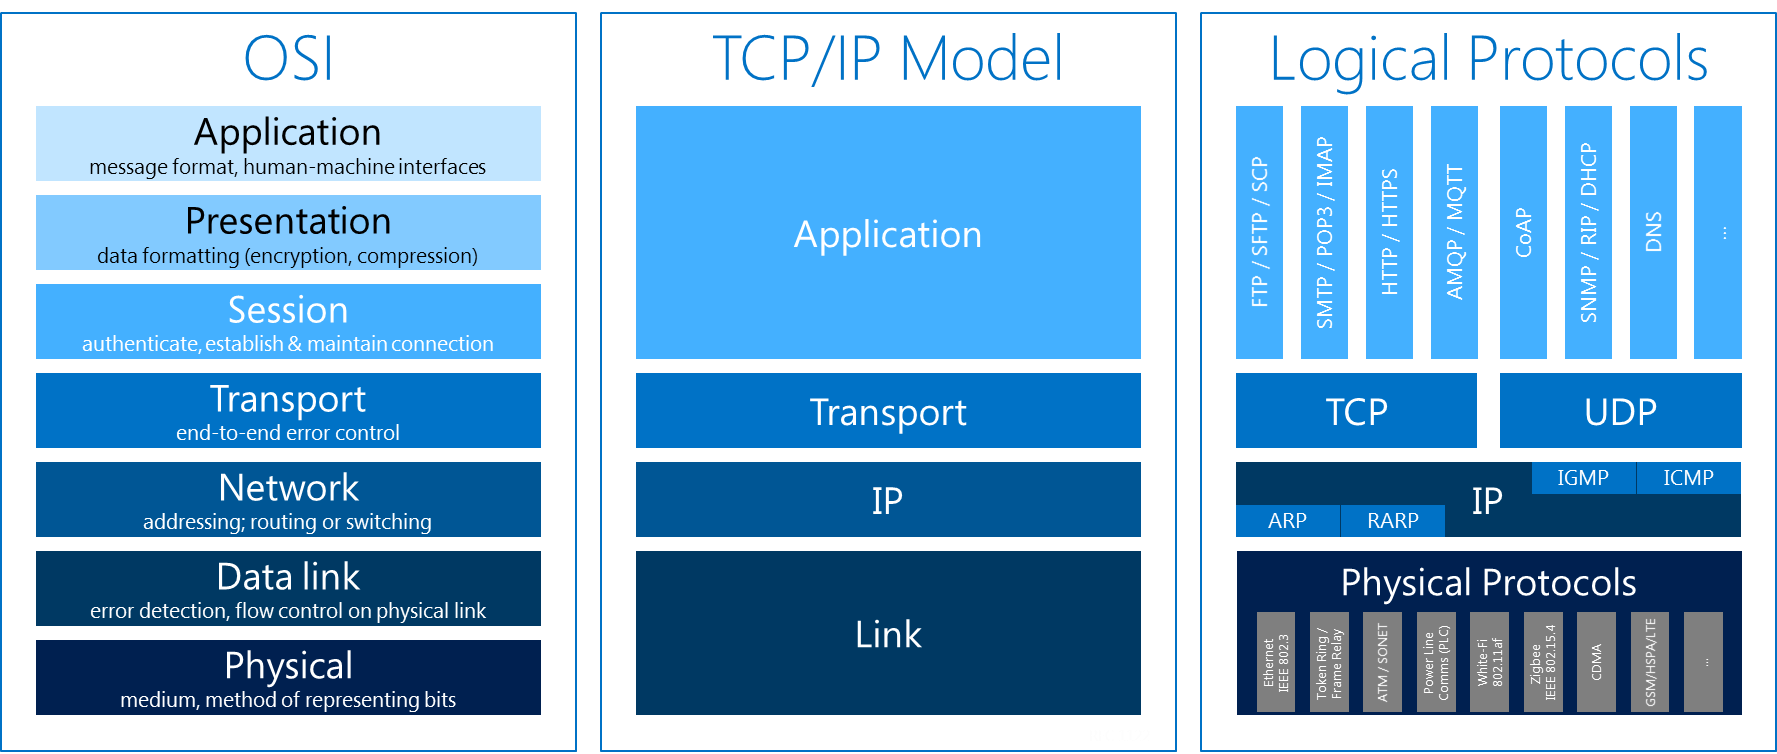
\includegraphics[width=0.8\linewidth]{images/loadbalancing3.jpg}
		\caption{OSI Modell \cite{LoadBalancingGrafik2}}
		\label{OSI Modell}
	\end{center}
\end{figure}

\subsection{Load Balancing auf verschiedenen Layern}
\label{sec:Load Balancing auf verschiedenen Layern}
Layer-2 Load Balancing (auch als Link- oder Portaggregation bezeichnet) verbindet zwei oder mehrere Links zu einer leistungsfähigeren logischen Verknüpfung. Aggregierte Verknüpfungen stellen zusätzlich Redundanz und Fehlertoleranz, wenn jeder der einzelnen aggregierten Links einen unterschiedlichen physikalischen Pfad folgt. Linkaggregation kann verwendet werden um den Zugang zu öffentlichen Netzwerken zu verbessern durch aggregieren von Modemverbindungen oder Digitalleitungen. 

Layer 4 Load Balancing ist für die Verteilung der Anfragen zu den Servern auf Transport Layer Ebene zuständig, dazu gehören die Transportprotokolle TCP, UDP und SCTP. Der Load Balancer verteilt die Netzwerkverbindung der Clients, die nur die IP-Adresse für einen Services wissen, an alle verfügbaren Server die für den Service zuständig sind.  

Das Konzept von Layer 7 (auch als Application-Level Load Balancing bezeichnet) ist die Lastenverteilung bezogen auf den Content-Typ (z.B. Scripts wie HTML, CSS, etc.) der Client-Anfrage. Geräte, die Layer 7 Load Balancing betreiben können, heißen Application Delivery Controllers (ADC). Da der Load Balancing Server weiß,  was der Client  für einen Content-Typ haben will, kann er abwägen,  welcher der vorhanden Server am besten mit dieser Anfrage umgehen kann, da jeder Content-Typ spezielle Anforderungen an Hardware und Software hat. \cite{LoadBalancing4}
\pagebreak
\begin{figure}[!ht]
	\begin{center}
		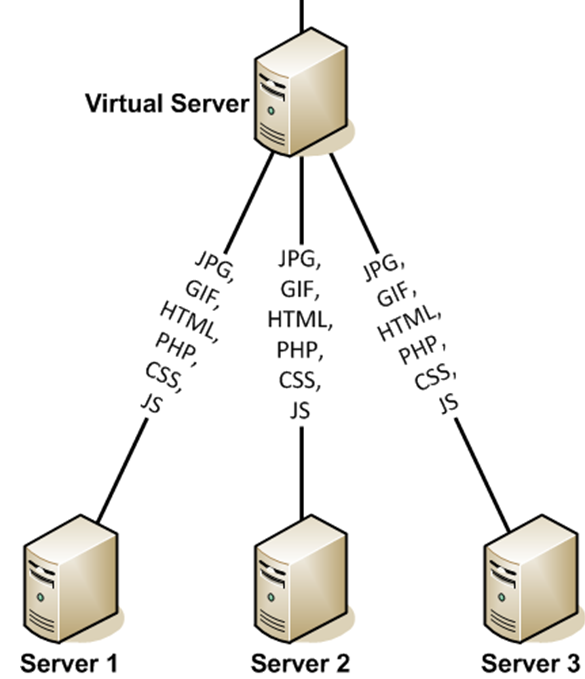
\includegraphics[width=0.3\linewidth]{images/loadbalancing4.jpg}
		\caption{Konzept Layer 7 Load Balancing \cite{LoadBalancing3}}
		\label{Konzept Layer 7 Load Balancing}
	\end{center}
\end{figure}

\textbf{Layer 7 Switching} \\
Layer 7 Switching (auch bezeichnet als Request oder Application Switching) verteilt Anfragen basierend auf Layer 7 Daten. Ein Layer 7 Switch ist für die Außenwelt ein Virtueller Server der Anfragen annimmt und diese Aufgrund von Richtlinien der Applikationen an die Server verteilt. Das heißt man kann die Server für spezielle Arten von Content optimieren, z.B. ein Server ist für Bilder optimiert und ein weiterer ist für Skriptsprachen optimiert. Im Unterschied zu Load Balancing muss nicht jeder Server alle Arten von Content zur Verfügung stellen, sondern kann sich auf eine Art von Content spezialisieren um die bestmögliche Performance zu erreichen. \cite{LoadBalancing3}

\begin{figure}[!h]
	\begin{center}
		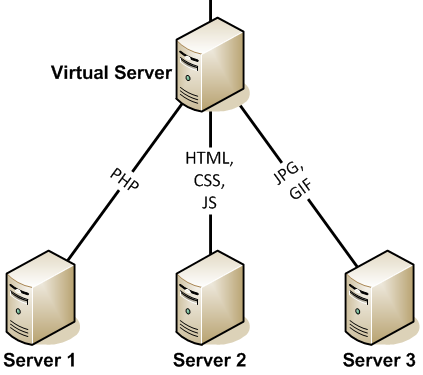
\includegraphics[width=0.3\linewidth]{images/loadbalancing5.jpg}
		\caption{Layer 7 Switching \cite{LoadBalancing3}}
		\label{Layer 7 Switching}
	\end{center}
\end{figure}

\textbf{Layer 7 Load Balancing} \\
Verbindet man das Load Balancing Konzept von Layer 7 mit Layer 7 Switching so erhält man Layer 7 Load Balancing. Layer 7 Switching allein reicht nicht aus, da wenn ein Server ausfällt, ein Typ von Content nicht mehr zur Verfügung gestellt werden kann. Deswegen erstellt man Pools von Servern, die auf einen Typ von Content spezialisiert sind. So ist man vor Ausfällen geschützt. 
\pagebreak
\begin{figure}[!h]
	\begin{center}
		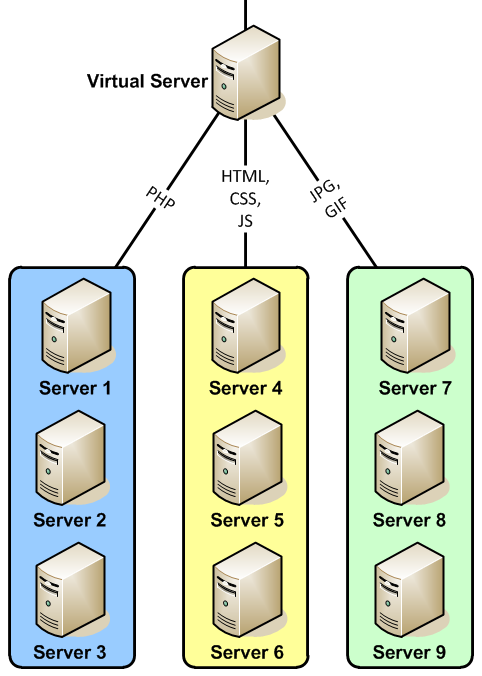
\includegraphics[width=0.3\linewidth]{images/loadbalancing6.jpg}
		\caption{Layer 7 Load Balancing \cite{LoadBalancing3}}
		\label{Layer 7 Load Balancing}
	\end{center}
\end{figure}

Layer 7 Load Balancing erhöht die Effizienz der Applikationsinfrastruktur. Dadurch dass der ADC den Content-Typ der Anfrage weiß kann er diese an den Server weiterleiten, der am besten mit diesem Content umgehen kann aufgrund der Serverhardware. \cite{LoadBalancing3}

\begin{figure}[!h]
	\begin{center}
		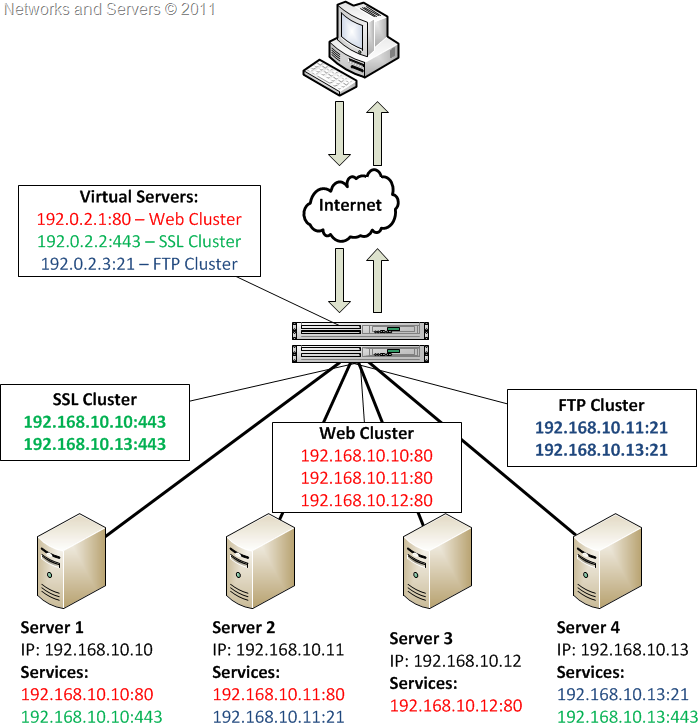
\includegraphics[width=0.55\linewidth]{images/loadbalancing7.jpg}
		\caption{Layer 7 Load Balancing \cite{LoadBalancing2}}
		\label{Layer 7 Load Balancing_2}
	\end{center}
\end{figure}

\pagebreak
\subsection{Paketfluss bei Load Balancing}
\label{sec:Paketfluss bei Load Balancing}

Bevor man sich den Paketfluss bei Load Balancing anschaut, sollte man sich kurz in Erinnerung rufen, wie TCP funktioniert. Eine TCP Verbindung involviert einen sogenannten „Three-Way Handshake“. Beispiel: Datenaustausch zwischen Client und Server. Zuerst sendet der Client ein SYN Paket zu dem Server (beinhaltet Source IP-Adresse, Source Portnummer, Ziel IP-Adresse und Ziel Portnummer). Wenn der Server dieses Paket erhält, sendet er eine SYN ACK an den Client. Der Client antwortet mit ACK, was bedeutet, dass der Verbindungsaufbau erfolgreich war. Jetzt können über diese Verbindung Daten zwischen Client und  Server ausgetauscht werden. Jede TCP Verbindung ist durch Source IP-Adresse, Source Portnummer, Ziel IP-Adresse und Ziel Portnummer eindeutig identifizierbar. Wenn der Datenaustausch beendet ist sendet der Client ein FIN Paket und der Server antwortet mit einer FIN ACK. Dadurch wird die TCP Verbindung beendet. \cite{LoadBalancing2}

\begin{figure}[!h]
	\begin{center}
		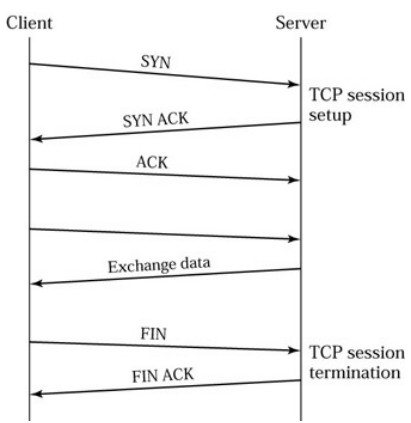
\includegraphics[width=0.6\linewidth]{images/loadbalancing9.jpg}
		\caption{TCP Three-Way Handshake \cite{LoadBalancing2}}
		\label{TCP Three-Way Handshake}
	\end{center}
\end{figure}

\pagebreak
\begin{figure}[!h]
	\begin{center}
		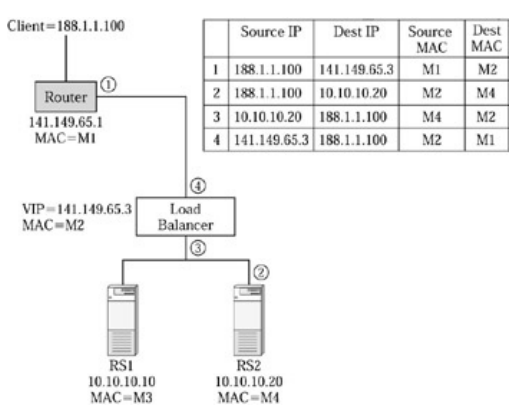
\includegraphics[width=0.45\linewidth]{images/loadbalancing10.jpg}
		\caption{TCP Three-Way Handshake \cite{LoadBalancing2}}
		\label{TCP Three-Way Handshake_2}
	\end{center}
\end{figure}
Paketfluss bei Load Blanancing anhand eines Beispiels (Load Balancer und zwei Webserver)
Der Client erzeugt eine TCP Verbindung, sendet eine http-Anfrage, erhält eine Rückmeldung und schließt die TCP Verbindung. Wenn der Load Balancer die erste TCP SYN Anfrage bekommt, enthält diese folgende Informationen:
\begin{enumerate}
\item Source IP Addresse = Client IP Addresse
\item Source Port = Port Nummer, die vom Client benutzt wird für diese TCP Verbindung
\item Destination IP Addresse = virtuelle IP, welche die Server Farm repräsentiert
\item Destination Port = Standardport 80 für Webserver
\end{enumerate}
Bevor dieses TCP SYN Paket erhalten wird, entscheidet der Load Balancer z.B. die Anfrage an Server RS2 weiterzuleiten. Damit der Server RS2 das Paket verarbeiten kann, muss die Destination IP Adresse die IP Adresse des Servers RS2 sein. Das heißt der Load Balancer ändert die virtuelle IP auf die IP Adresse des Servers RS2 bevor das Paket weitergeleitet wird.   
Wenn der User die Domain dieser Seite aufruft, macht der Browser eine DNS Anfrage um die virtuelle IP der Domain zu bekommen. Der Browser vom Client sendet ein TCP SYN Paket um eine neue TCP Verbindung zu erzeugen. Wenn der Load Balancer dieses TCP SYN Paket erhält identifiziert er dieses als Kandidat für Load Balancing (da das Paket eine virtuelle IP enthält). Da diese Verbindung neu ist und noch keine Einträge im Session Table vorhanden sind, identifiziert der Load Balancer die zwei Server RS1 und RS2 als mögliche Kandidaten für eine neue Verbindung. Aufgrund des ausgewählten Scheduling Algortihmus entscheidet sich der Load Balancer welcher Server besser geeignet ist. Nehmen wir in diesen Fall an das Server RS2 ausgewählt wurde. Sobald der Zielserver ausgewählt wurde, erzeugt der Load Balancer einen neuen Session Eintrag im Session Table und ändert die Destination IP- und MAC Adresse auf jene von Server RS2. Wenn RS2 sich mit TCP SYN ACK rückmeldet, erreicht das Paket den Load Balancer (Source IP von RS2, Destination IP von Client). Danach ersetzt der Load Balancer die IP Adresse von RS2 mit der virtuellen IP und leitet das Paket an den Router weiter und schließlich zum Client. Wenn die Verbindung mit FIN oder RESET beendet wird, löscht der Load Balancer den Session Eintrag aus dem Session Table. \cite{LoadBalancing2}

\subsection{Health Checks}
\label{sec:Health Checks}

Health Checks sind notwendig, damit der Load Balancer nicht Anfragen an fehlerhafte Server versendet. Das kann auch bedeuten das der Server zwar verfügbar ist, jedoch aber die Applikation fehlerhaft ist oder das die Applikation korrupten Content zur Verfügung stellt. Load Balancer können diese Fehler erkennen und die Anfragen zu anderen funktionierenden Servern weiterleiten ohne manuelles Eingreifen des Administrators. Es gibt zwei Kategorien von Health Checks, nämlich die sogenannten in-band- und out-of-band checks. Bei in-band-checks kontrolliert der Load Balancer einfach den normalen Netzwerkverkehr um zu kontrollieren, ob der Server intakt ist. Out-of-band Health Checks jedoch werden explizit vom Load Balancer durchgeführt.\vspace{5mm}

\textbf{Grundlegende Health Checks} \\

Load Balancer können zumindest bestimmte Netzwerk-Level Checks auf verschiedenen OSI-Layern durchführen. Bei einem Layer 2 Health Check wird eine Address Resolution Protocol (ARP) Anfrage verwendet, um die MAC Adresse einer gegebenen IP Adresse herauszufinden. Der Server wird auf diese ARP Anfrage reagieren, es sei denn er funktioniert nicht. Bei einem Layer 3 Health Check wird die reale IP-Adresse des Servers gepingt um herauszufinden ob der Server läuft. Bei Layer 4 Health Checks versucht der Load Balancer sich zu einem spezifischen TCP oder UDP Port zu verbinden auf der eine Applikation läuft. Der Load Balancer sendet eine TCP SYN Anfragen zu dem spezifischen Port und wartet auf eine TCP SYN ACK Rückmeldung. Falls der Load Balancer diese Rückmeldung nicht erhält, wird der Port als down markiert. Jeder Port wird vom Load Balancer unabhängig behandelt, so kann es sein das ein Port down ist, alle anderen jedoch erreichbar sind. Sämtliche Applikationen die auf erreichbaren Ports laufen sind weiterhin verfügbar, der Load Balancer markiert nur Applikationen als down, die nicht verfügbar sind.\vspace{5mm}

\textbf{Applikationsspezifische Health Checks} \\

Load Balancer können auch Layer 7 Health Checks für weit verbreitete Applikationen durchführen.  Bei Webserver kann der Load Balancer eine HTTP GET Anfragen für eine URL versenden und durch zusätzliche Konfiguration die HTTP Rückgabecodes kontrollieren, so kann z.B. ein 404 Fehler entdeckt werden. Bei DNS kann der Load Balancer DNS Lookup Abfragen versenden (für das Auflösen von Domainnamen zu IP-Adresse) um die Resultate mit dem erwarteten Ergebnis zu vergleichen.\vspace{5mm}

\textbf{Applikationsabhängigkeiten} \\

Bei Verwendung von mehreren Applikationen die voneinander abhängig sind kann der Load Balancer das Feature Port Grouping verwenden, wodurch mehrere TCP oder UDP Ports zu Gruppen zusammengefasst werden. Wenn nur einer dieser Ports nicht funktioniert, wird alle Applikationen der Gruppe als down makiert.\vspace{5mm}
\pagebreak

\textbf{Content Checks} \\

Um den Inhalt zu kontrollieren gibt es mehrere Möglichkeiten: 
\begin{list}{•}{}
\item Nach Keywords suchen
\item Checksum berechen und mit dem konfigurierten Wert vergleichen
\item Load Balancer konfigurieren, sodass er HTTP GET Anfragen für eine bestimmte URL versendet. Ein Script/Programm das am Server läuft führt eine Vielzahl an Health Checks durch. Falls alle Health Checks erfolgreich waren, erzeugt das Script/Programm die vorher konfigurierte URL, sonst wird diese gelöscht. \cite{LoadBalancing2}
\end{list}

\subsection{Sicherheit}
\label{sec:Sicherheit}

Da Load Balancer das Front End der Server Farm sind, können Load Balancer die Server vor Angriffen schützen. Viele Load Balancing Produkte sind mittlerweile schon mit mehreren Sicherheitsfeatures ausgestattet. Den Servern der Server Farm können private IP Adresse vergeben werden, um direkten Zugriff von außen zu unterbinden. Um mit Hosts, die eine private IP Adresse haben, zu kommunizieren, muss man zuerst über ein Gerät geleitet werden, welches NAT durchführt. \cite{LoadBalancing2}  

\subsection{Ausfallsicherheit}
\label{sec:Ausfallsicherheit}  
Ein großer Vorteil von Load Balancing ist die Ausfallsicherheit. Wenn ein Server ausfällt, übernehmen einfach die anderen verfügbaren Server die Anfragen. Doch was ist wenn der Load Balancer ausfällt? Ein einzelner Load Balancer ist ebenfalls ein Single Point of Failure, das heißt wenn der Load Balancer ausfällt ist der gesamte Service/Dienst nicht verfügbar. Durch Verwendung von zwei Load Balancern kann man dieses Problem lösen. Bei Einsatz von zwei Load Balancern gibt es zwei mögliche Konfigurationen, nämliche Active-Standby und Active Active. Bei der Active-Standby Variante verteilt der aktive Load Balancer die Anfragen und der passive Load Balancer agiert als Backup. Bei der Active-Active Variante verteilen beide Load Balancer die Anfragen und agieren als Backup für den jeweilig anderen Load Balancer.\vspace{5mm}

\textbf{Active-Standby} \\ 

Die aktive Einheit verteilt den Netzwerkverkehr auf die vorhandenen Server, der Passive reagiert auf keine Anfragen. Die zwei Load Balancer sind über einen private Link miteinander verbunden und kontrollieren mittels eines speziellen Protokolls den Zustand des jeweils anderen Load Balancers. Wenn der aktive Load Balancer ausfällt springt die passive Einheit sofort ein.
\pagebreak
\begin{figure}[!h]
	\begin{center}
		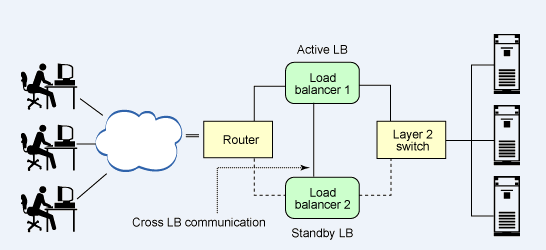
\includegraphics[width=0.6\linewidth]{images/loadbalancing13.png}
		\caption{Active-Standby Variante \cite{LoadBalancingGrafik3}}
		\label{Active-Standby Variante}
	\end{center}
\end{figure}


\textbf{Active-Active} \\

Bei der Active-Active Variante verteilen beide Load Balancer die Anfragen und agieren als Backup für den anderen Load Balancer. Damit man die Active-Active Variante verwenden kann, gibt es mehrere Möglichkeiten. Eine davon ist die Verwendung von mehreren VIPs. Falls einer der Load Balancer ausfällt, übernimmt die noch funktionierende Einheit auch die VIP des ausgefallenen. Jetzt muss nur noch ein Weg gefunden, wie die Anfragen auf die beiden Load Balancer verteilt werden. Dafür kann man DNS verwenden, dass die Web Domain zu einer IP-Adresse entschlüsselt und ein Round-Robin zwischen den beiden VIPs durchführt, damit beide Load Balancer Anfragen erhalten.  
\begin{figure}[!h]
	\begin{center}
		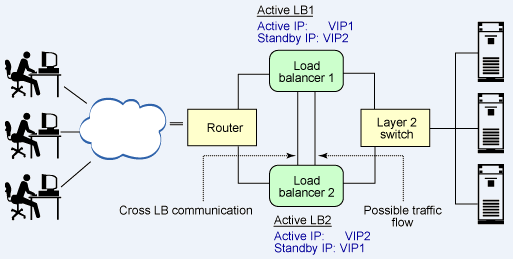
\includegraphics[width=0.6\linewidth]{images/loadbalancing14.png}
		\caption{Active-Active Variante \cite{LoadBalancingGrafik3}}
		\label{Active-Active Variante}
	\end{center}
\end{figure}

\pagebreak
\section{URL Switching}
\label{sec:URL Switching}

URL Switching ist notwendig, wenn ein einzelner Server nicht den gesamten Content eines Services zur Verfügung stellen kann (wegen zu geringer Speicherkapazität). Durch URL  Switching kann der Content auf mehrere Server aufgeteilt werden. Zusätzlich können Server, welche die gleiche Art von Content zur Verfügung stellen zu Gruppen zusammengefasst werden. Durch definieren von URL Regeln und URL Switching Richtlinien (Policies) kann man festlegen, wie der Load Balancer den Content auf die Server Gruppen aufteilt.\vspace{5mm}

\textbf{Aufteilen von statischen und dynamischen Content} \\

Eine andere Möglichkeit von URL Switching ist die Aufteilung von statischen und dynamischen Content auf den Server Gruppen. Der statische Content ändert sich relativ selten und ist auch einfach zu verwalten. Der dynamische Content aber ändert sich sehr oft und hängt auch teilweise von der Useranfrage ab. 
Ein Beispiel für dynamischen Content ist eine Google Suchanfrage. Wenn man nach z.B. Systemtechnik sucht sieht die URL der Ergebnisseite folgendermaßen aus: 
www.google.com/?.....q=Systemtechnik
Das q steht für das Skript bzw. Programm des Google Webservers, welches den Inhalt nach dem ? (in diesem Fall Systemtechnik) als Input entgegennimmt. Dieses Programm generiert auf Basis meines Inputs die Suchergebnisse.
Man kann URL Regeln für den Load Balancer definieren, welche statischen und dynamischen Content auf die ausgewählten Server Gruppen aufteilen.\vspace{5mm}

\textbf{URL Switching Nutzungsrichtlinien} \\

Wenn man URL Switching verwendet um die richtige Server Gruppe für die Verarbeitung auszuwählen, sollte man die Session Persitence innerhalb der Gruppe gewährleisten. Das kann durch die Verwendung von Cookie Switching in Kombination mit URL Switching erreicht werden. Durch die Cookie-Read Methode wird vom Server ein Cookie eingefügt, welches vom Load Balancer gelesen werden kann. Wenn das Cookie existiert sendet der Load Balancer die Anfrage zu dem vom Cookie angegebenen Server. Falls das Cookie nicht existiert verwendet der Load Balancer die definierten URL Switching Regeln um die Anfrage an die passende Server Gruppe zu versenden. \cite{LoadBalancing2}

